
\chapter{Florestas Aleatórias}

\begin{citacao}
	``Todos os modelos estão errados, mas alguns são úteis.''  - George Box
\end{citacao}

Neste capítulo desenvolvemos o modelo de floresta aleatória partindo de primeiros princípios. Primeiro veremos algumas definições e conceitos centrais ao Aprendizado de Máquina supervisionado, depois os conceitos de teoria dos grafos que sustentam Árvores de Decisão e discutir brevemente sua estimação. Por fim veremos quais propriedades indesejáveis desses modelos nos levam a construir florestas aleatórias. 

\section{Noções de Aprendizado de Máquina Supervisionado}

Primeiro precisamos de algumas definições caras ao contexto de Aprendizado Supervisionado. Uma \textbf{observação} é um par de realizações de duas variáveis aleatórias. O par consiste em $x \in \R^k$, contendo $k$ \textbf{variáveis explicativas} e $y \in \R$ que chamaremos de \textbf{variável resposta}. Com algumas convenções é possível representar dados não-numéricos. Variáveis binárias podem ser representadas por pares $0$ e $1$, então usar 'apenas' números reais não é uma grande limitação. O conjunto de vetores possíveis de serem medidos, o produto cartesiano de todos os espaços amostrais das variáveis aleatórias contidas no vetor com variáveis explicativas, é o \textbf{Espaço de Mensuração} $\mathcal{X}$ e $\mathcal{Y}$ o \textbf{Espaço de Resposta}, equivalente ao espaço amostral da variável resposta. Por exemplo: se uma dimensão deste espaço representa idade, entendemos que seu suporte está nos inteiros positivos entre $0$ e, digamos, $120$. Se uma variável é uma categoria binária, então seu suporte está em $0$ e $1$. 

Munido de dados relacionando mensurações de variáveis e explicativas e com uma resposta a ser estudada, um modelador está interessado em um algoritmo que relacione medidas dentro de $\X$ com previsões para valores plausíveis de $\Y$. Essa representação matemática representando regras de previsão é o objeto fundamental do Aprendizado de Máquinas.

\begin{defi}[Modelos]
Um \textbf{modelo} é uma função $f: \mathcal{X} \to \mathcal{Y}$. Se $\mathcal{Y}$ é enumerável dizemos que é um modelo de \textbf{Classificação}, se for um subconjunto convexo da reta real dizemos que é de \textbf{Regressão} e, em particular no caso em que $\Y = [0, \,1]$, dizemos ser de \textbf{Risco}. A derivada $\frac{\partial f}{\partial x}, \, x \in \mathcal{X}$, se existir, é dita o \textbf{efeito marginal} da variável em relação a que se diferencia $f$.
\end{defi} 

Classificar um paciente como sendo ou não portador de uma doença é  um problema de classificação binária. Classificar o tipo de câncer a partir de medidas de um tumor é um problema de classificação multiclasse. Estimar o preço de um imóvel com base em suas características é um problema de regressão. Estimar a \textit{probabilidade de default}  de um empréstimo é um problema de risco, embora estimar se o empréstimo irá ou não entrar em default seja, novamente, um problema de classificação binária. 

Ao definir um modelo não fizemos grandes hipóteses sobre $f$, apenas que se for diferenciável, sua derivada é uma grandeza de interesse. Temos infinitos modelos para qualquer problema de modelagem não-trivial, todos candidatos válidos. Dentro dessa enorme variedade de modelos alguns são florestas aleatórias, outros são de regressões lineares. O que se faz ao estimar um modelo é escolher, na classe de modelos que o procedimento de estimação comporta, o mais apropriado aos dados. Ao estimar uma árvore de decisão jamais obteremos um modelo de regressão linear, e vice-versa. Exatamente o que configura um modelo apropriado aos dados é uma questão que será discutida mais à frente.

Algumas propriedades interessantes de um modelo, como, por exemplo, são trivialmente obtidas em modelos de regressão linear. Basta diferenciar um polinômio. Essa propriedade não vale em funções definidas em trechos, como veremos que uma Floresta Aleatória é. Efeitos parciais são centrais para várias aplicações de econometria e demandam uma maneira de aproxima-los em outras classes, potencialmente mais interessantes que os lineares, de modelos. 

\section{Um pouco de Teoria dos Grafos}

Vamos estabelecer alguns fatos básicos de Teoria dos Grafos, caracterizar árvores nesse contexto e oferecer um resultado com duas condições razoavelmente fracas e suficientes para estabelecer que um grafo é uma árvore. A apresentação seguirá \citeonline{chartrand2013first}. Para um tratamento alternativo e mais amplo de Teoria dos Grafos o leitor pode verificar \citeonline{bollobas2013modern}.

\begin{defi}[Grafos]
Um \textbf{grafo} é um par $G = (V, E)$, onde $V$ é um conjunto de elementos que chamamos \textbf{vértices} e os de $E$, \textbf{arestas}. Se uma aresta conecta dois vértices, dizemos ser aresta incidente aos vértices. Notamos o conjunto de vértices incidentes a uma aresta $h$ pela função $\phi(h)$. O número de arestas que se liga a um vértice $v$ é chamado de seu \textbf{grau}.
\end{defi}

\begin{defi}[Rotas em Grafos]
Um \textbf{passeio} é qualquer sequência de arestas $(h_1, h_2, ..., h_{n-1})$ para os quais há uma sequência de vértices $(v_1, v_2, ..., v_n)$ de forma que $\phi(h_i) = \{v_i, v_{i+1}\}$. Uma \textbf{trilha} é um passeio em que toda aresta é distinta. Um \textbf{caminho} é uma trilha em que todo vértice é distinto. Um \textbf{ciclo} é qualquer trilha que comece e termine no mesmo vértice. Um grafo que não admite ciclos é dito \textbf{acíclico}.
\end{defi}

\begin{defi}[Conexidade]
Um grafo $G$ é dito \textbf{conexo} se para qualquer par de vértices $x, y \in V \subset G$ há pelo menos um caminho cujo vértice inicial é $x$ e o terminal é $y$. Um subconjunto de vértices de um grafo desconexo em que vale esta propriedade é dito um \textbf{componente}.
\end{defi}


\begin{defi}[Árvores]
Um grafo $G$ é dito uma \textbf{árvore} se para quaisquer dois vértices de $G$ existe um caminho único os ligando. Podemos escolher um vértice arbitrário e defini-lo como a \textbf{raiz} da árvore. Os vértices que não são a raiz e têm grau unitário são ditos \textbf{folhas}. Os com grau maior que $1$ que não são a raiz são chamados \textbf{nodos}. Um conjunto disjunto de árvores é dito uma \textbf{floresta}.
\end{defi}


\begin{figure}[H]
    \centering
    \captionbox{Da esquerda para a direita: grafo conexo, um desconexo e uma árvore.}{ 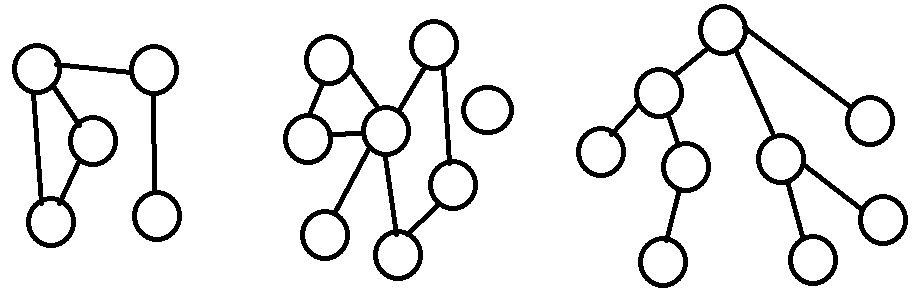
\includegraphics[scale = .55]{imagens/grafos.png}}
       \label{fig:grafos}
    \fonte{Elaboração Própria}
\end{figure}

A Figura 1 ilustra algumas das definições anteriores. O resultado a seguir é interessante para nossa aplicação porque ilustra duas propriedades úteis de árvores.

\begin{teo}
$G$ é uma árvore se, e somente se, é conexo e acíclico.
\end{teo}

\begin{prova}

Seja $G$ uma árvore. $G$ é trivialmente conexo, pois por definição existe um caminho entre qualquer par de vértices. Suponha por absurdo que $G$ admita um ciclo. Então existe uma trilha começando e terminando em um vértice $v$ de $G$. Escolha um vértice qualquer $u$ desse ciclo. Então existe um caminho $v \to u $ e uma trilha (possivelmente um caminho) $u \to v$. Dois casos ocorrem:

\begin{itemize}
    \item Se $u \to v$ é uma trilha, é também a união de dois caminhos $u \to w$ e $w \to v$. Note que nesse caso podemos truncar o caminho $v \to u$ em $w$ e estabelecemos dois caminhos distintos entre $v$ e $w$. Em contradição com $G$ ser uma árvore.

    \item Se $u \to v$ é um caminho então a contradição é imediata, pois existiriam dois caminhos entre $u$ e $v$.
\end{itemize}


Agora a volta. Tome $G$ conexo e acíclico, escolha dois vértices $v$ e $u$. Suponha por absurdo que exista mais de um caminho entre $v$ e $u$. Então necessariamente existe ciclo no grafo $G$, basta 'ir' por um caminho e 'voltar' por outro. $G$ é uma árvore.
$\blacksquare$
\end{prova}

%Uma propriedade interessante de árvores, e que ilustra como testes seguidos são excludentes entre sim, é: 

%\begin{teo}
%Seja $G$ uma árvore. Para qualquer par de vértices $u$, $v$ existe uma aresta $h$ tal que $G - \{h\}$ é igual à união de dois grafos disjuntos $G_1$ e  $G_2$,  $u \in G_1$ e $v \in G_2$.
%\end{teo}

%\begin{prova}
%Seja $G$ uma árvore, escolha dois vértices $v \neq u$ com um caminho os ligando que passa por $h$. Suponha por absurdo que $G - \{h\}$ é conexo. Então existiam pelo menos dois caminhos entre $v$ e $u$. Se existiam dois caminhos distintos o grafo $G$ não era uma árvore. 
%\end{prova}


\section{Construindo Modelos com Árvores}

Vamos agora cobrir duas situações hipotéticas que ilustram como essas definições aparecem em um contexto mais aplicado.

\subsection{Classificação Binária}

 A unidade de email marketing de uma grande empresa de e-commerce quer segmentar clientes entre entusiastas de tecnologia, que engajarão felizmente com campanhas de aparelhos novos, e usuários relutantes de tecnologia, que não precisam receber esse contato nas suas caixas de email. Uma equipe selecionou algumas centenas de clientes aleatoriamente e manualmente os classificou usando entrevistas e análise de histórico de compras, um processo caro, demorado e de profundidade. Cabe agora a um analista tentar reproduzir os esforços manuais e não-escaláveis da equipe em um modelo preditivo que pode ser aplicado na base verdadeira de clientes usando os resultados do estudo.

O analista consultou o banco de dados da empresa e montou uma amostra contendo os seguintes dados: idade do cliente, percentual das compras em eletrônicos, valor médio da compra. Estamos falando de um espaço de mensuração $\X \subset \R^3$. Como a variável resposta é binária, $\Y = \{0, 1\}$. 

Um procedimento possível seria primeiro estimar por mínimos quadrados generalizados um modelo para probabilidade uma observação pertencer a uma classe $f: \R^3 \to [0, \, 1]$ e depois alguma maneira de traduzir uma probabilidade presumida pelo modelo a uma classe $g: [0, \, 1] \to \{0, 1\}$. O modelo final, neste caso, seria a composição $g \circ f: \R^3 \to \{0, 1\} $.

Modelos têm hipóteses. Nesse caso uma delas é que as variáveis explicativas são independentes, no sentido de que sua distribuição conjunta é apenas o produto de suas distribuições marginais. A intuição do analista diz haver interações entre renda e idade, por exemplo. Um público mais velho que faz grandes compras em eletrônicos provavelmente é tão entusiasta quanto estudantes universitários que compram quase exclusivamente eletrônicos. O analista então pode seguir por outro caminho e enumerar uma série de perguntas sobre cada observação antes de emitir um julgamento:

\begin{itemize}
    \item O cliente tem menos de 30 anos?
    \item Mais de um quarto das compras desse cliente foram em eletrônicos?
    \item A compra média desse cliente é maior que 250 reais?
\end{itemize}

Cada pergunta aqui pode ser lida como uma função. 'O cliente tem menos de $k$ anos?' é, computacionalmente,  $f: \R^2_+ \to \{0, 1\}$. Algumas perguntas são mais informativas que outras. Afinal, um usuário teve mais de 90\% das compras em eletrônicos é quase certamente um entusiasta de tecnologia, enquanto saber que um usuário tem mais de 20 anos provavelmente não é tão informativo. 

Ao compor perguntas sucessivamente chegamos a uma espécie de fluxograma de decisão. Uma boa previsão de perfil para clientes, por exemplo, com menos de 30 anos que compram eletrônicos em 60\% das compras passadas e gastam 40\% a mais que a média por compra provavelmente é que são usuários ávidos de tecnologia. Ao passo que um usuário de 72 anos que teve 10\% das compras em eletrônicos e faz compras 40\% menores que a média provavelmente não. Note, no entanto, que um usuário idoso que compra apenas eletrônicos na plataforma muito provavelmente é entusiasta. A composição das repostas é importante.

Supondo que toda pergunta seja sim ou não e que toda observação tenha uma resposta para toda pergunta, acabamos com uma estrutura recursiva. Nenhuma resposta individual altera as outras. Podemos elaborar com isso um fluxograma que tem a estrutura de um grafo árvore, representado graficamente na Figura 2. 


\begin{figure}[H]
    \centering
    \captionbox{Um exemplo de árvore de decisão.}{ 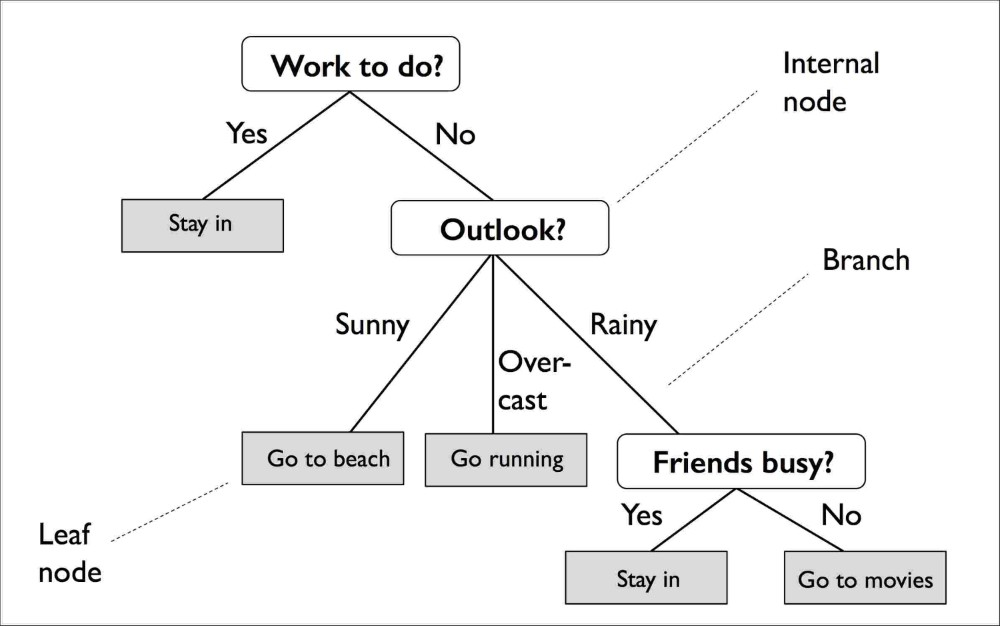
\includegraphics[scale = .55]{imagens/arvore.png}}
        \label{fig:arvore}
    \fonte{Elaboração Própria}
\end{figure}

Recapitulando: a composição de perguntas e suas combinações distintas de respostas levam a uma partição do espaço de mensuração. Cada partição é associada a uma regra de previsão/ classificação. Podemos representar essa lógica com uma árvore. O modelo resultante é a função definida por trechos que atribui a cada região do espaço de mensuração uma regra de previsão. Formalmente:


\begin{defi}[Modelos de Árvore]
Seja $\X, \Y$ um par de espaços de mensuração e resposta. Uma \textbf{Árvore de Decisão} é uma função definida por trechos $\A: \X \to \Y$, onde $\Y$ é enumerável. No caso em que $\Y$ ao, ao invés de enumerável, um subconjunto convexo da reta chamamos \textbf{Árvore de Regressão}. Se $\Y = [0, 1]$ é comum se referir a uma \textbf{Árvore de Risco}.
\end{defi}


\subsection{Regressão}

Uma empresa de tecnologia no setor imobiliário quer trabalhar em um modelo de precificação de aluguel. A ideia é que donos de imóveis recebam um valor sugerido compatível com o mercado e embutir isso no serviço.
 
 Um analista coletou dados de aluguel e algumas informações básicas do apartamento. Área, número de quartos, de banheiros, se aceita animais, se é mobiliado e em qual cidade está localizado. A Tabela 1 contém médias para as variáveis mais relevantes, por cidade.
 
 
\begin{tabular}{l|r|r|r|r|r|r|r|r}
\hline
cidade & area & quartos & banheiros & vagas & andar & mobiliado & aluguel & aceita\_animal\\
\hline
Belo Horizonte & 136.71745 & 2.863596 & 2.167405 & 1.7245350 & 3.514615 & 0.1302037 & 2765.900 & 0.7307352\\
\hline
Porto Alegre & 93.27658 & 2.086430 & 1.652550 & 0.9749352 & 3.949006 & 0.2644771 & 2069.884 & 0.8461538\\
\hline
Rio de Janeiro & 93.14216 & 2.158964 & 1.657563 & 0.6792717 & 5.247899 & 0.2626050 & 2774.703 & 0.8011204\\
\hline
São Paulo & 124.69289 & 2.395466 & 2.204030 & 1.6002713 & 5.608216 & 0.2600271 & 3600.296 & 0.7512110\\
\hline
\end{tabular}




 
\begin{figure}[H]
    \centering
    \captionbox{Um exemplo de árvore de regressão.}{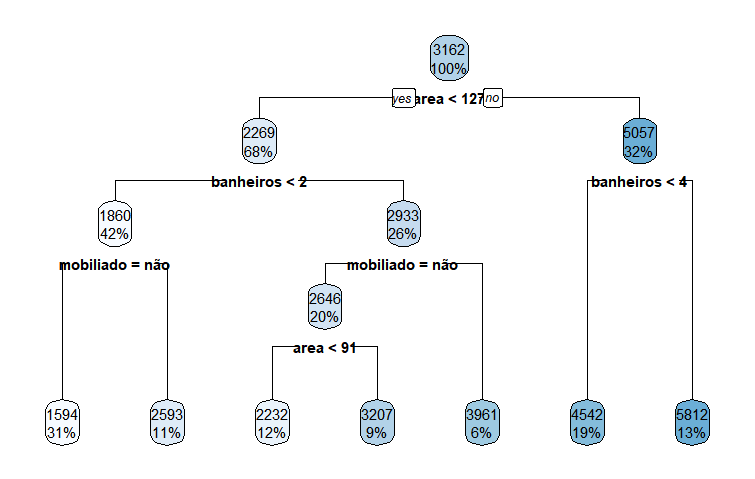
\includegraphics[scale = .70]{imagens/arvore_decisao_houses.png}}
        \label{fig:arvore_reg}
    \fonte{Elaboração Própria}
\end{figure}

A Figura 3 mostra a árvore de regressão estimada. As porcentagens se referem à fração da amostra original que passa pelos testes até ali, o número é a média da variável resposta no grupo. Com as regras de previsão que estimamos, um apartamento com mais de 127 m$^2$ e mais de 4 banheiros tem aluguel presumido de 5812 reais. Já o aluguel de um com área menor, menos de 2 banheiros e sem mobília é presumido em 1594 reais.
 
 
\section{Noções de Estimação de uma Árvore de Decisão}

Nessa seção veremos como traduzir uma amostra $A$ em uma árvore de decisão $\A$ Uma abordagem candidata é o procedimento original apresentado na primeira edição de \citeonline{breiman1984classification}. Imagine que temos uma massa de dados, uma nuvem de pontos em algum espaço de mensuração. Vamos elaborar uma enorme lista de sequência de perguntas, avaliar qual sequência é mais informativa e usar a sua árvore como modelo. Podemos avaliar o quão informativa é uma sequência de perguntas com partição recursiva:

\begin{defi}
Um algoritmo de divisão de conjuntos que opere dividindo em subconjuntos os resultantes no passo anterior é dito uma \textbf{Partição Recursiva}. Toda partição recursiva pode ser representada com uma árvore. O número perguntas a ser feito, a métrica de qualidade de cada pergunta e, opcionalmente outros parâmetros como um critério para um valor mínimo da métrica de qualidade para aceitar uma pergunta, são ditos \textbf{hiperparâmetros}.
\end{defi}

Cada sequência de perguntas pode ser entendida como uma sequência de testes $\tau_i$, a partição induzida pelas perguntas sendo representada por uma árvore $\A$ onde todo vértice que não seja uma folha tem um $\tau_i$ associado. Estimar a árvore é encontrar quais são as perguntas mais apropriadas, dado uma amostra. 

Começamos com a amostra completa e enunciamos uma série de perguntas sobre ela — um procedimento computacionalmente intensivo por isso a estimação é quase sempre estocástica. Um subconjunto aleatório das perguntas possíveis é testado. Escolhemos a pergunta que melhor performa e partimos para os nodos ''filhos''. Repetimos o processo em cada um até algum gatilho ser ativado, então usamos o grupo para definir a regra de classificação/previsão. Em classificação podemos usar a classe mais comum no grupo, em regressão podemos usar a média ou mediana da variável resposta no grupo. Três gatilhos usuais:

\begin{itemize}
    \item \textbf{Nenhum teste cumpre um valor mínimo para a métrica de qualidade} \newline Cada pergunta respondida diminui a informação disponível, tornando o ganho de informação decrescente. Alguma hora, a cargo do modelador definir, uma pergunta adicional provavelmente custa mais em parcimônia e computação do que devolve em acurácia de previsão. É hora de gerar uma folha.
    
    \item \textbf{O número de perguntas feitas chegou ao máximo} \newline
    Uma maneira de forçar parcimônia do modelo é limitar o número de perguntas. Algumas implementações diferenciam o número total de perguntas do número de perguntas sucessivas.  
    
    \item \textbf{O número de observações do nodo não cumpre um mínimo} \newline 
    A amostra que chegou no nodo está abaixo de um mínimo. Por ser um dos mais simples e ter uma relação diretamente proporcional com o número de regras de previsão/classificação distintos é um dos mais comuns na literatura.
\end{itemize}

É esse o procedimento. Dividimos a amostra guiados por alguma métrica de sucesso e usamos a divisão final como um modelo estimado contendo regras de previsão/classificação informadas pelos dados. Resta entender o que queremos dizer, rigorosamente, com um teste ser \textit{melhor} que outro.


\subsection{Métricas de Informação}

Voltando ao primeiro exemplo, a pergunta ''usuário tem mais de 90\% das compras em eletrônicos?'' provavelmente segrega muito bem as classes. É difícil conceber que um usuário assim não seja entusiasta de eletrônicos, ou pelo menos sustente alguém que é. Ela não é, no entanto, parcimoniosa. O tamanho do grupo de clientes que retorna positivo para essa pergunta dificilmente será relevante por isso essa pergunta provavelmente não será um bom insumo para uma regra de classificação. Pense também no grupo que \textbf{não} retorna positivo. Ele é provavelmente pouco segregado. Uma pergunta ''melhor'', espera-se, renderia dois grupos bem segregados e de tamanhos não muito díspares. 

Começando pelo contexto de classificação, suponha $J$ classes. Uma primeira métrica que respeita esse equilíbrio entre divisão e parcimônia é o \textbf{Ganho de Informação} \cite{kullback1951information}. Podemos expressa-lo como a diferença entre a entropia do nodo ''pai'' da divisão e a soma ponderada da entropia nos nodos filhos. 

O vetor $P(n_i) = (p_1, p_2, ..., p_J)$ representa as probabilidades de que um elemento aleatoriamente escolhido do grupo que chegou no nodo $n_i$ seja da $i$-ésima classe. A entropia do nodo $n_i$ é $H(n_i) = - \sum_{p_j \in P(n_i)} p_j \log_2 p_j$. Defina $H(n_i \, | \, a), H(n_i \, |\,  b)$ como a entropia dos potenciais nodos filhos de $n_i$, dado um teste $\tau$ que gere dois grupos $a$ e $b$. Defina $P_a(\tau), P_b(\tau)$ como a proporção de elementos do nodo pai que vai para cada filho dado um teste $\tau$. 

Então o ganho de informação por entropia $\I_E(\tau)$ é dado por $\I_E(\tau) = H(n_i) - P_a(\tau) \,H(n_i \, |\,  a) - P_b(\tau)\, H(n_i \, |\,  b)$. Em cada divisão, usando essa métrica, escolhemos $\tau^* = \argmax{\I_E(\tau)}$.  Outra métrica de classificação é a \textbf{Impureza de Gini} \cite{strobl2009introduction}, definida como $\I_G(\tau) = \sum_{i = 1}^J p_i ( 1  - p_i) =  1 - \sum_{i = 1}^J p_i^2$.





 \section{Construindo uma Floresta Aleatória}
 

Uma limitação do modelo construído até aqui é que ele é inclinado a \textit{overfitting}, quando o modelo performa muito bem nos dados em que treinou e muito mal em dados novos. O problema é notoriamente acentuado em contexto de regressão. Afinal, um modelo de árvore parcimonioso terá algo entre 3 e 20 regras de previsão distintas, ao passo que um modelo linear cobre uma região convexa. 

Isso deve a modelos de árvore serem modelos de alta variância: mudanças pequenas nos dados de treino podem gerar regras de previsão vastamente diferentes. Em compensação isso os torna modelos de baixo viés, capturam muito bem padrões nos dados apresentados. Ao contrário de modelos lineares, que tipicamente irão produzir previsões de variância mais baixa que modelos de árvore e com mais viés porque não conseguem incorporar relações latentes entre variáveis explicativas. 

Essa troca entre viés e variância é uma espécie de restrição fundamental da modelagem e permeia Aprendizado de Máquina. O \textbf{\textit{trade-off} viés-variância} é um conjunto de resultados para uma variedade de classes de modelos. Várias formulações desse resultado podem ser encontradas em \citeonline{derumingy}.

Podemos realizar uma simulação de Monte Carlo para por esse problema em perspectiva. No próximo capítulo exploraremos melhor modelos lineares e sua estimação por Mínimos Quadrados Ordinários (OLS). Agora, vamos ilustrar dois comportamentos desagradáveis dos modelos de árvore disponíveis até aqui, é para mitiga-los que vamos dar o próximo passo. 

Voltando ao exemplo da árvore de regressão para preços de casas. Vamos agora selecionar aleatoriamente várias amostras de apartamentos e treinar uma árvore e um modelo linear (estimado por OLS) em cada. Como comparativo, vamos prever o aluguel de um apartamento de $82m^2$, $2$ quartos, $1$ banheiro, no Rio de Janeiro, não-mobiliado e aceite animais com cada um dos modelos e observar como as previsões se distribuem, como mostramos na Figura 4.

\begin{figure}[H]
    \centering
    \captionbox{A distribuição das previsões por classe de modelo.}{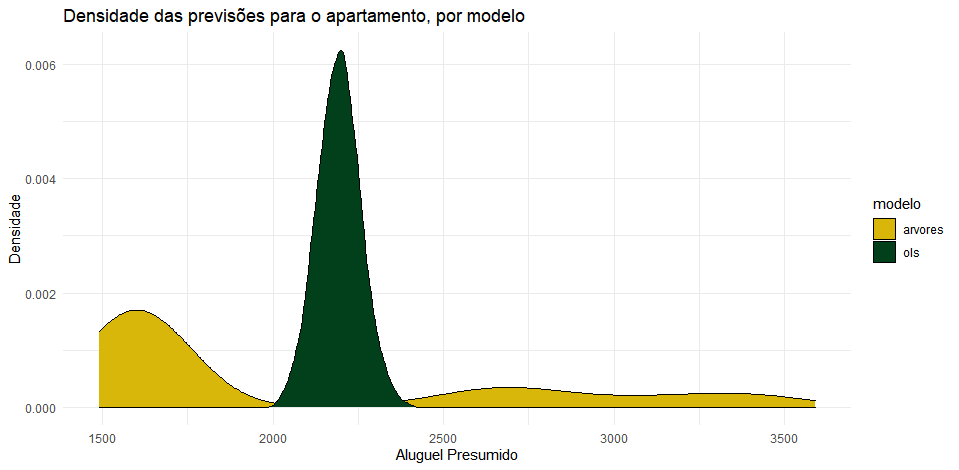
\includegraphics[scale = .60]{imagens/exemplo_var_arvores.png}}
        \label{fig:arvore_var_ols}
    \fonte{Elaboração Própria}
\end{figure}


O que acontece se ao invés de treinarmos \textbf{uma} árvore, treinar \textbf{várias} e usar a alguma agregação das previsões individuais como previsão final? Em caso de classificação basta usar a moda, em caso de regressão basta usar a média. Sabemos pelo Teorema do Limite Central que a distribuição desse modelo seria normal, ao contrário do que acontece com a distribuição das previsões de uma árvore individual. 

\begin{teo}[Lindenberg-Lévy]
Seja $(\textbf{X}_1, ..., \textbf{X}_n)$ uma amostra independente e identicamente distribuída com $\E[\textbf{X}_i] = \mu$ e $\V[\textbf{X}_i] = \sigma^2 < \infty$. Então:

\begin{align}
    \sqrt{n}\,(\bar{\textbf{X}_i }- \mu) \xrightarrow[n \to \infty]{d} N(0, \sigma^2)
\end{align}

\end{teo}

\begin{prova}
Ver \citeonline{basu1980rate}.
\end{prova}

Agregar várias árvores não irá diminuir em absoluto a variância das previsões, temos modelos de baixo viés, mas as dará propriedades estatísticas mais amigáveis. Talvez melhor ainda, fará com que as previsões de um modelo de regressão passem a ocupar uma região convexa, assim como em modelos lineares. Podemos definir modelos de florestas aleatórias formalmente, como em \citeonline{hastie2015statistical} agora.

\begin{defi}
Considere uma função $\mu : \R^m \to \R$ e uma floresta $\F' = \{\A_1, ..., \A_m\}$. Uma \textbf{Floresta Aleatória} é um modelo $\F : \X \to \Y$,  $x \mapsto \mu(\A_1(x), ..., \A_m(x))$. 
\end{defi}
















 %\begin{defi}
 %Seja $A$ uma instância de um Banco $(\mathcal{X}, \C)$. Existe um conjunto de subamostras únicas dessa instância, $B = \{ B_1, B_2, ..., B_k\}$  independentes. Treine em cada elemento de $B$ uma árvore de decisão $\A_i$ e chame de $F(x)$ o conjunto de imagens obtidas ao aplicar cada $\A_i$ a uma observação $x$ da instância $A$. Uma \textbf{Floresta Aleatória} é um classificador $\F : F(x) \to \C$. 
  %\end{defi}
  
  %\begin{defi}
 % Seja $A$ uma instância de um Banco $(\mathcal{X}, \C)$ com $n$ observações. Seja $F$ um conjunto de $k$ árvores de decisão treinadas em $A$ de acordo com a definição anterior. Seja $x_i$ a $i$-ésima observação da instância $A$ e, por fim, $\1(\cdot)$ a função indicadora. A \textbf{Margem} da floresta aleatória $\F$ formada pelas árvores de decisão $\A_j$ na observação $x_i$ é a função $M(\F, x_i) := \sum_{j=1}^k \1 ( \A_j (x_i) = \C(x_i) ) - \sum_{j=1}^k \1  ( \A_j (x_i) \neq \C(x_i) )$.
 % \end{defi}
  
 
 % \begin{defi}
 %Para uma observação $x$ de uma instância $A$, o \textbf{Erro de Generalização} $G(\F, x) := \Prob (M(\F, A, x)) < 0)$.  \end{defi}
  
 % A margem provê uma medida do quão precisa é a floresta em votar corretamente na classe verdadeira da observação. Uma margem maior sinaliza uma maior capacidade da floresta de discriminar o dado observado entre possíveis classes.  

 %\begin{teo}[Convergência do Erro de Generalização] Seja $A$ uma instância de um Banco $(\mathcal{X}, \C)$. Defina a sequência $E_k = \{ G(\F_k, A, x) \}$ de forma que $\F_k = \F_{k-1} \bigcup \A_k $,  Tome as classes possíveis $\C = \{1,2,3,...,c,...,J \}$ e uma observação $x$, tal que $\C(x) = c$. Então $E_k \to \sum_{i=1}^k \1 ( \A_i (x) = c ) - \underset{}{\text{Max}} \sum_{i=1}^k \1  ( \A_i (x) \neq c) $
 
% \end{teo}
 
%Alguns refinamentos muito interessantes podem ser feitos. \textit{Bagging}, a ideia de expor árvores diferentes da floresta à observações e variáveis explicativas diferentes. \textit{Boosting}, treinar uma árvore no resíduo de outra, fazendo a floresta aprender lentamente, incorporando padrões mais sutis. 
 
 
 
% \begin{prova}
% Ver o Apêndice 1 de \citeonline{breiman2001random}. \blacksquare
% \end{prova}
